\section{Введение}
%Модель Изинга используется для моделирования и изучения термодинамических свойств. Поведение структуры в модели Изинга сильно зависит от её геометрии. Так например на одно мерных моделях не происходит фазовый переход, но на двумерных моделях переход есть. Но что происходит в промежуточных размерностях? Например если взять какую-то последовательность узлов на двумерной решётке. Именно это и является главным вопросом в данном проекте. 
В данном проекте проводится исследование модели Изинга на фиксированной двумерной конформации. 

Возьмём конформацию(связанную не само пересекающуюся последовательность узлов) на двумерной решётке. Такие конформации можно рассматривать как термодинамическую систему, основанную на модели Изинга, для которых существуют две фазы: плотная(глобулярная) и развёрнутая. Эти фазы соответствуют низким и высоким температурам системы.

\begin{figure}[h]
	\centering
	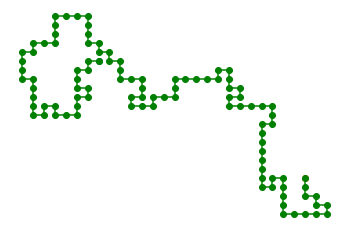
\includegraphics[width=0.45\textwidth]{../images/loose_conf.png}
	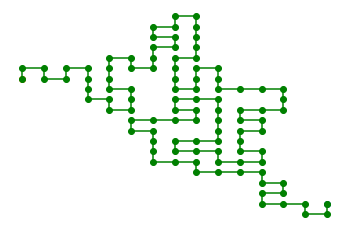
\includegraphics[width=0.45\textwidth]{../images/dense_conf.png} 
	\caption{Пример неплотной и плотной конформации}
\end{figure}

Если посмотреть на изображения конформаций каждого вида, хорошо видно, что плотные конформации по структуре близки с двумерным решёткам, где у каждого узла имеется множество соседей, и развёрнутые конформации наоборот близки к одномерным структурам, где узлы у которых больше 2 соседей встречаются редко. Соответственно можно предположить, что плотные конформации будут иметь свойства схожие с двумерными решётками, а развёрнутые с одномерными.


\subsection{Модель изинга}
Будем рассматривать конформацю как модель Изинга. В каждом узле конформации размещён спин $s_i$ принимающий значения $+1, -1$. Внешнее поле отсутствует. Гамильтониан системы $H = -J\sum_{i, j} s_i s_j$ где $i, j$ индексы соседних узлов, $J$ - коэффициент взаимодействия.

\subsection{Метод Монте-Карло}
Для моделирования системы используется метод Монте-Карло. Мною были реализованы версии с односпиновым и кластернным апдейтом, однако для измерений я использовал кластерную версию. Благодаря отказоустойчивости она работает значительно быстрее, и быстрее сходится, особенно при низких температурах.

На каждой итерации мы выбираем случайный спин и начиная с него начинаем строить кластер из одинаково направленных спинов, добавляя новые спины в кластер с определённой вероятностью. затем мы меняем значения спинов в кластере на противоположные.